\documentclass[10pt,a4paper]{article}
\usepackage[utf8]{inputenc}
\usepackage[T1]{fontenc}
\usepackage{amsmath}
\usepackage{amssymb}
\usepackage{graphicx}
\usepackage[english,russian]{babel} 
\usepackage{fontspec} 
\setmainfont{Times New Roman}
\title{Отчет по лабораторной работе №3 и №4}
\author{Ивлев А.Е Б19-511}
\usepackage{graphicx}
\graphicspath{{./Graphics/}}
\DeclareGraphicsExtensions{.pdf,.png,.jpg,.eps}
\begin{document}
	\maketitle
	
	\begin{figure}[h]
		\centering
		{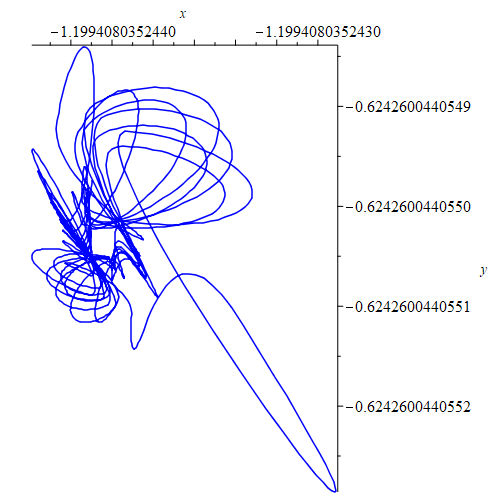
\includegraphics[scale=0.2]{Lab3 f=0}}
		{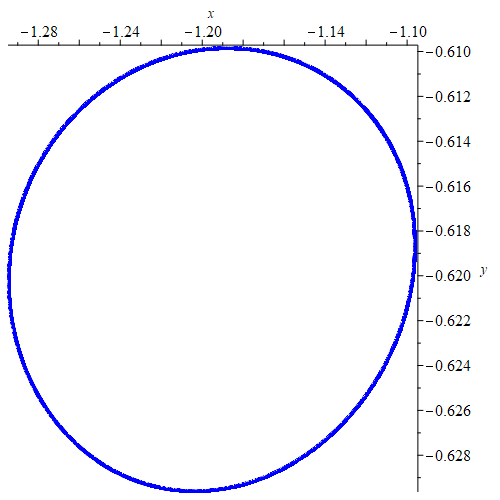
\includegraphics[scale=0.2]{Lab3 f=0.1}}
		{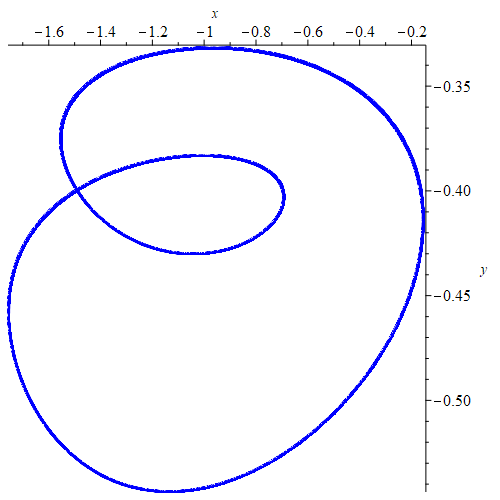
\includegraphics[scale=0.2]{Lab3 f=0.65}}
		{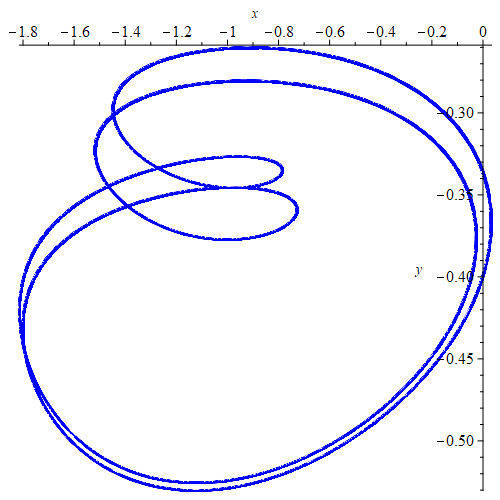
\includegraphics[scale=0.2]{Lab3 f=0.7}}
		{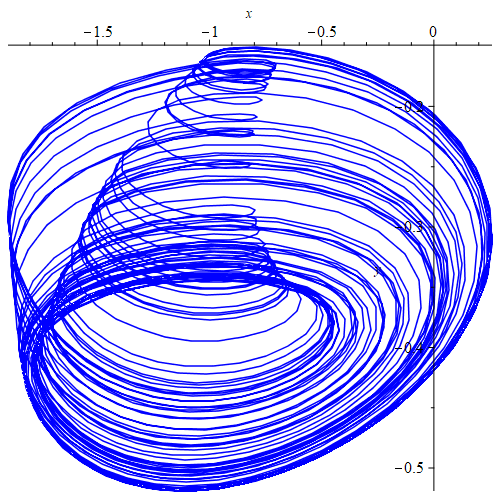
\includegraphics[scale=0.2]{Lab3 f=0.745}}
		{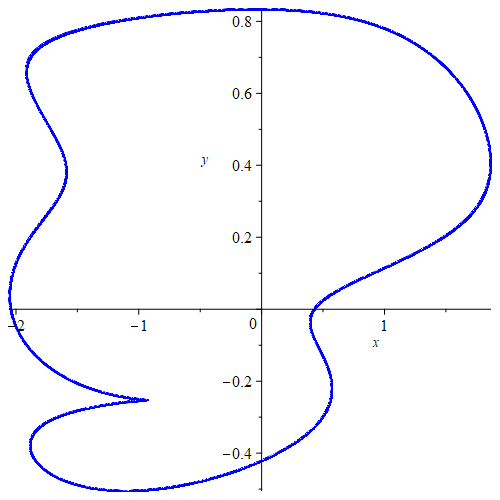
\includegraphics[scale=0.2]{Lab3 f=0.8}}
		{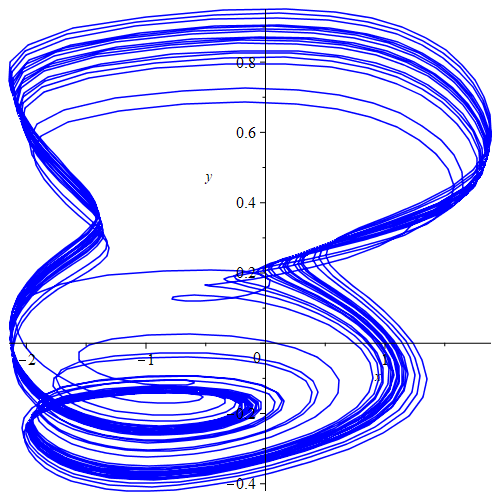
\includegraphics[scale=0.2]{Lab3 f=1.1}}
		{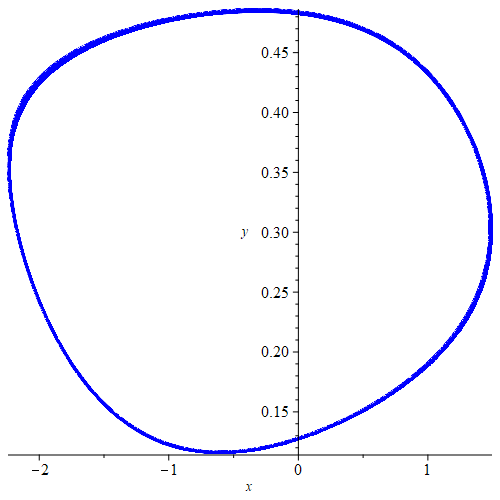
\includegraphics[scale=0.2]{Lab3 f=2}}
		\caption{Фазовые портреты при $f = 0$, $f = 0.1$, $f = 0.65$, $f = 0.7$, $f = 0.745$, $f = 0.8$, $f = 1.1$, $f = 2$}
		\label{image/1}
	\end{figure}

	\begin{figure}[h]
		\centering
		{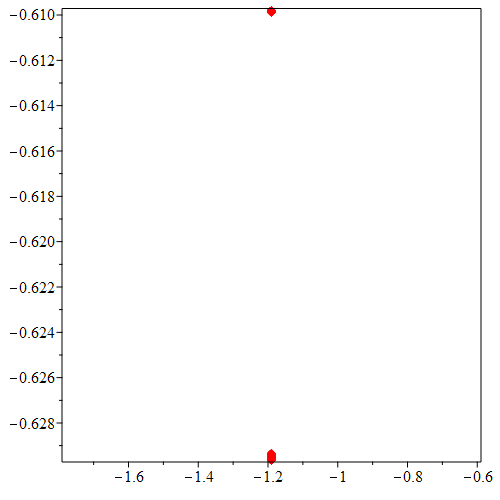
\includegraphics[scale=0.2]{poincare f=0.1}}
		{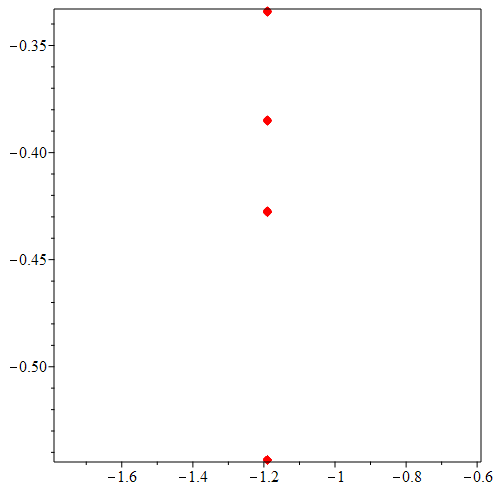
\includegraphics[scale=0.2]{poincare f=0.65}}
		{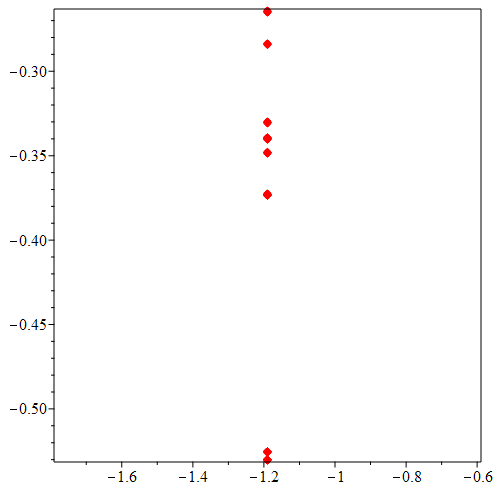
\includegraphics[scale=0.2]{poincare f=0.7}}
		{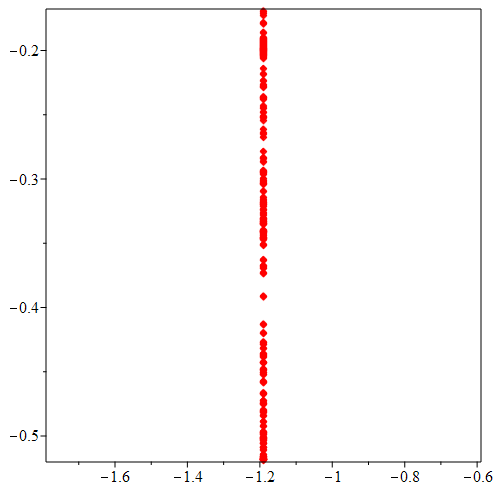
\includegraphics[scale=0.2]{poincare f=0.745}}
		{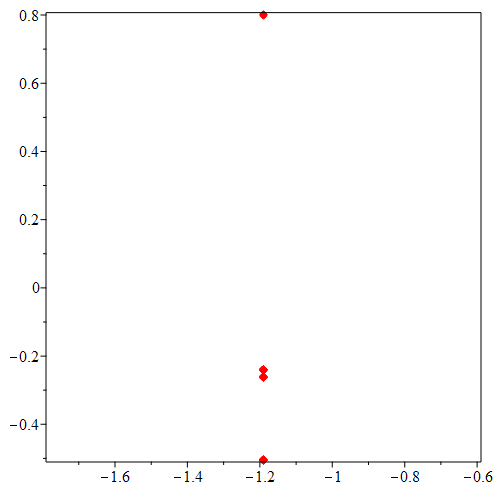
\includegraphics[scale=0.2]{poincare f=0.8}}
		{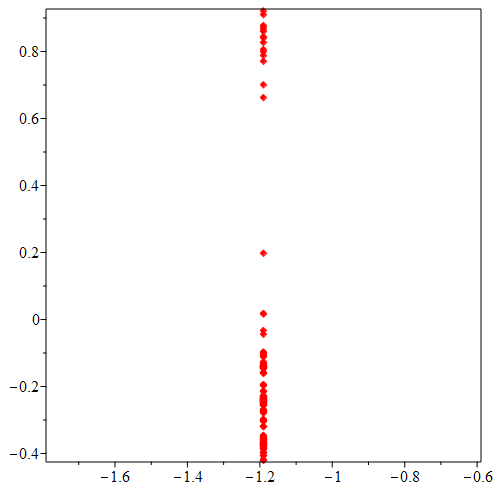
\includegraphics[scale=0.2]{poincare f=1.1}}
		{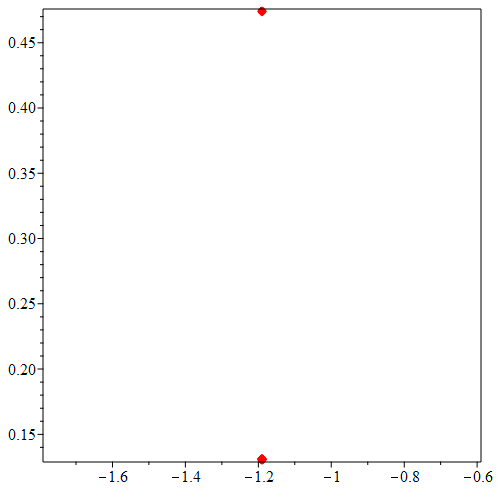
\includegraphics[scale=0.2]{poincare f=2}}
		\caption{Сечение Пуанкаре (прямая $x = -1.19$) при $f = 0.1$, $f = 0.65$, $f = 0.7$, $f = 0.745$, $f = 0.8$, $f = 1.1$, $f = 2$}
		\label{image/2}
	\end{figure}

	\begin{figure}[h]
		\centering
		{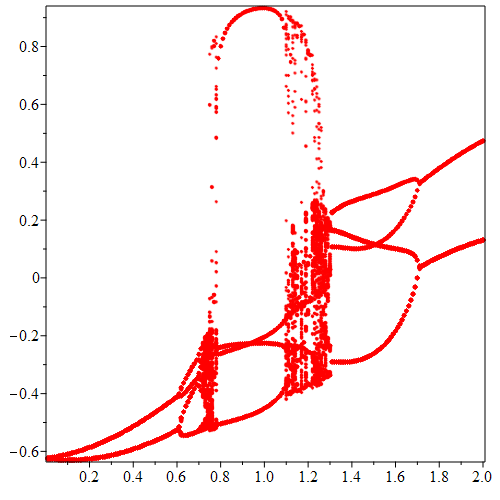
\includegraphics[scale=0.5]{bifurcation 0.01}}
		\caption{Бифуркационная диаграмма}
		\label{image/2}
	\end{figure}

	\begin{figure}[h]
		\centering
		{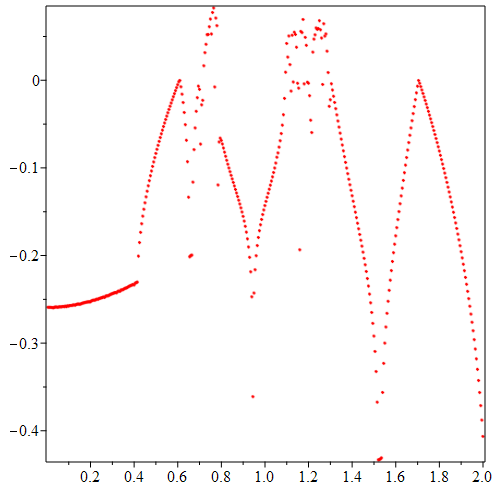
\includegraphics[scale=0.2]{lyapunov1 0.005}}
		{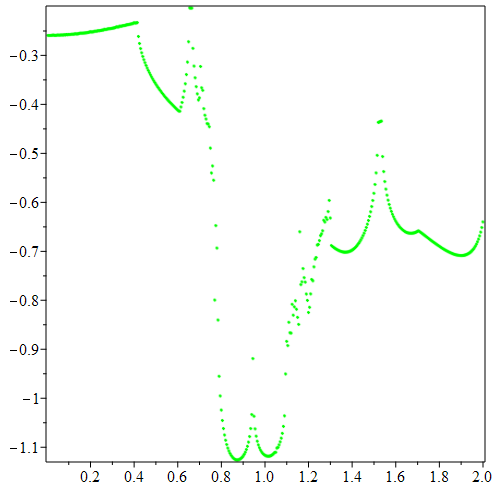
\includegraphics[scale=0.2]{lyapunov2 0.005}}
		{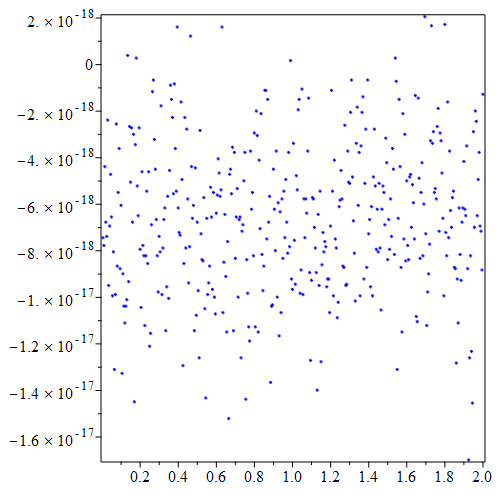
\includegraphics[scale=0.2]{lyapunov3 0.005}}
		\caption{Показатели Ляпунова}
		\label{image/2}
	\end{figure}

	Исходная динамическая система:

	\begin{equation}
		\label{math/1}
		\begin{cases}
			\dot{x} = x - \frac{x^3}{3} - y + f \cos \omega t, \\
			\dot{y} = c(x+a-b y).
		\end{cases}
	\end{equation}

	Значения параметров: $a = 0.7, b =0.8, c =0.1, \omega = 1, f \in [0; 2]$. Система решается с нулевым начальным условием.

	При увеличении параметр $f$ возникает бифуркация удвоения периода, ведущая к хаотическому поведению.
	
	\begin{equation}
		\label{math/1}
		x = 
		\begin{cases}
			\ \exp(-\frac{1}{(x-2)^2} - \frac{1}{(x-1)^2}), 1 < x < 2\\
			\ -\exp(-\frac{1}{(x)^2} - \frac{1}{(x-1)^2}), 0 < x < 1\\
			\ 0, x={0, 1, 2}.
		\end{cases}
	\end{equation}
	
\end{document}